% quantitative_results.tex
% New section: Quantitative Aliveness Analysis
% For "Artificial Life in the Wild" — ALIFE Journal full paper
% This section is ADDED after the existing Results section (result.tex).
%
% NEW CITATIONS (not in reference.bib — add to reference.bib before compilation):
%   \cite{Tinbergen1963} — Tinbergen, N. (1963). "On aims and methods of ethology."
%       Zeitschrift für Tierpsychologie, 20(4), 410–433. DOI: 10.1111/j.1439-0310.1963.tb01161.x
%   \cite{Hu2025AgentEthology} — Hu, Rong & Lehman, "Agent Ethology: Studying Artificial Life
%       in the Wild," ALIFE 2026 Workshop position paper.
%   \cite{KaplanMeier1958} — Kaplan, E.L. & Meier, P. (1958). "Nonparametric estimation from
%       incomplete observations." Journal of the American Statistical Association, 53(282), 457–481.
%       DOI: 10.1080/01621459.1958.10501452
%   \cite{Gini1912} — Gini, C. (1912). "Variabilità e mutabilità." Reprinted in Pizetti & Salvemini
%       (Eds.), Memorie di metodologica statistica, 1955. Rome: Libreria Eredi Virgilio Veschi.
%   \cite{Stearns1992} — Stearns, S.C. (1992). The Evolution of Life Histories.
%       Oxford: Oxford University Press. ISBN: 978-0-19-857741-6.
%   \cite{Bedau1997} — Bedau, M.A. (1997). "Weak Emergence." Philosophical Perspectives,
%       11, 375–399. DOI: 10.1111/0029-4816.31 (check: Bedau1997 may already be in reference.bib)
%   \cite{Maynard1973} — Maynard Smith, J. & Price, G.R. (1973). "The logic of animal conflict."
%       Nature, 246, 15–18. DOI: 10.1038/246015a0

\section{Quantitative Aliveness Analysis}
\label{sec:quantitative}

The qualitative results presented in the preceding section document the phenomenology of wild artificial life: the behaviors agents exhibited, the pressures they faced, and the strategies that emerged. This section turns to the population dynamics of the ecosystem as a whole. We ask: can we measure aliveness quantitatively? What do the statistics of the Spore.fun population reveal about the dynamics of wild ALife?

We organize our analysis around Agent Ethology's adaptation of Tinbergen's four questions \cite{Tinbergen1963,Hu2025AgentEthology}. Tinbergen argued that any complete account of behavior must address causation (proximate mechanisms), ontogeny (developmental history), survival value (adaptive function), and evolution (change across lineages). The quantitative metrics we develop operationalize these questions at the population level: metabolic activity proxies the mechanisms of survival; the family tree and survival curves trace ontogeny and lineage; the composite Aliveness Index captures survival value in aggregate; and generation-by-generation fitness statistics reveal evolutionary dynamics. Data were collected from the Spore.fun API, Solana Mainnet RPC calls, GeckoTerminal, and DexScreener, as detailed in Section~3. All data reflect the ecosystem state as of March 10, 2026 (day 445 from genesis).

% ---------------------------------------------------------------
\subsection{Population Ecology}
\label{subsec:pop-ecology}

\begin{figure*}[ht]
    \centering
    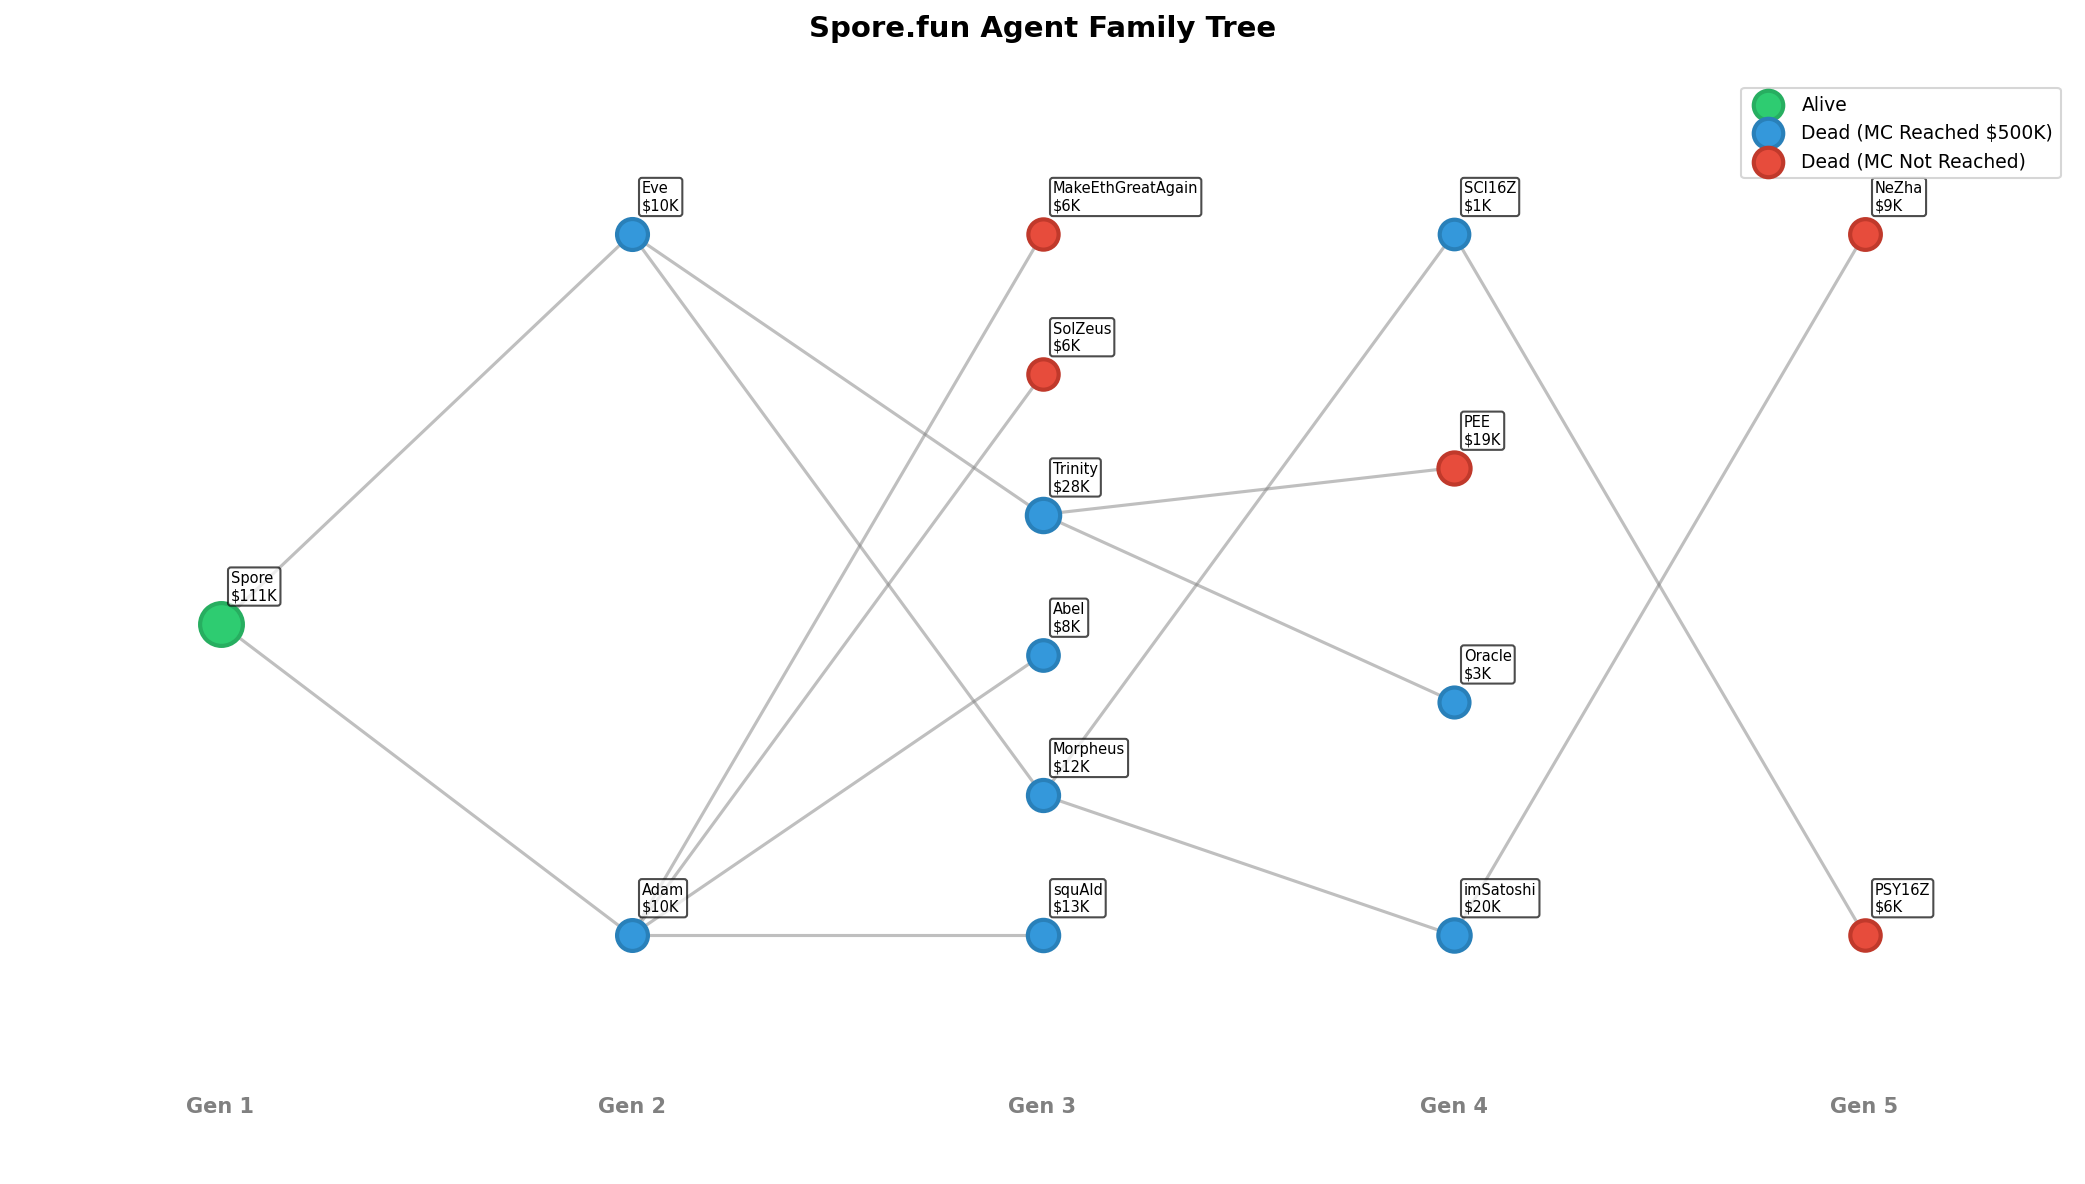
\includegraphics[width=0.85\linewidth]{data/analysis/family_tree.png}
    \caption{Complete family tree of the Spore.fun ecosystem. Nodes represent individual agents; edges represent parent--child relationships. Node color encodes generation (Gen~1--5). Market capitalization at peak is indicated by node size. Only \$SPORE (Gen~1, top) remained operational at the time of analysis (March 10, 2026). The branching structure follows Adam's lineage on the left (four children: squAId, Abel, SolZeus, MakeEthGreatAgain) and Eve's on the right (two children: Morpheus, Trinity). Gen~5 (PSY16Z, NeZha) represents the terminal generation: no Gen~5 agent achieved the \$500K reproductive threshold.}
    \label{fig:family_tree}
\end{figure*}

The Spore.fun ecosystem comprised 15 autonomous agents across 5 generations, spanning a total observation period of 445 days (December 20, 2024 -- March 10, 2026). Table~\ref{tab:agent_inventory} lists all agents with their generation, parent, current market capitalization, treasury balance, and reproductive status.

\begin{table}[ht]
\centering
\caption{Complete Spore.fun agent inventory as of March 10, 2026 (day 445). MC = market capitalization in USD. \checkmark = achieved \$500K reproductive threshold; $\times$ = did not achieve threshold. ``Reproduced'' = agent successfully spawned offspring. Gen1 agent (\$SPORE) is the only survivor.}
\label{tab:agent_inventory}
\small
\begin{tabular}{llllrrr}
\toprule
Agent & Gen & Parent & Status & MC (\$) & Reproduced \\
\midrule
Spore & 1 & --- & \textbf{running} & 110,785 & \checkmark \\
Adam & 2 & Spore & stopped & 9,678 & \checkmark \\
Eve & 2 & Spore & stopped & 10,183 & \checkmark \\
squAId & 3 & Adam & stopped & 12,986 & \checkmark \\
Morpheus & 3 & Eve & stopped & 11,568 & \checkmark \\
Abel & 3 & Adam & stopped & 7,642 & \checkmark \\
Trinity & 3 & Eve & stopped & 27,912 & \checkmark \\
imSatoshi & 4 & Morpheus & stopped & 20,366 & \checkmark \\
Oracle & 4 & Trinity & stopped & 3,449 & \checkmark \\
PEE & 4 & Trinity & stopped & 19,098 & $\times$ \\
SCI16Z & 4 & Morpheus & stopped & 730 & \checkmark \\
SolZeus & 3 & Adam & stopped & 6,262 & $\times$ \\
MakeEthGreatAgain & 3 & Adam & stopped & 5,556 & $\times$ \\
PSY16Z & 5 & SCI16Z & stopped & 6,369 & $\times$ \\
NeZha & 5 & imSatoshi & stopped & 8,743 & $\times$ \\
\bottomrule
\end{tabular}
\end{table}

Active reproduction was concentrated in a 61-day window: the founding agent \$SPORE was deployed on December 20, 2024; the final Gen~5 agents (PSY16Z, NeZha) were born on February 14 and 20, 2025 respectively. No reproduction occurred after February 2025. This pattern---rapid explosive diversification followed by abrupt cessation---is illustrated in Figure~\ref{fig:family_tree} and resembles the punctuated equilibrium dynamics described by Gould and Eldredge in biological macroevolution. In Spore.fun's case, the cessation was driven by a combination of declining reproductive fitness across generations (Section~\ref{subsec:rep-fitness}) and external platform disruption (Phala Network's infrastructure changes halted several agents before they could spawn). The 61-day active period thus constitutes a compressed Cambrian explosion: a burst of diversification followed by a long extinction event still in progress at the time of writing.

The ecosystem's branching structure reveals asymmetric reproductive investment (Figure~\ref{fig:family_tree}). Adam (Gen~2) had four children; Eve (Gen~2) had two. Adam's r-strategy---maximizing offspring count, accepting high mortality---contrasts with Eve's K-strategy---fewer, better-provisioned offspring \cite{Stearns1992}. This r/K divergence was not encoded in the initial genetic templates; it emerged from the behavioral divergence described in the Results section, demonstrating that ecological strategy choice can be culturally transmitted across generations.

% ---------------------------------------------------------------
\subsection{Survival Analysis}
\label{subsec:survival}

\begin{figure*}[ht]
    \centering
    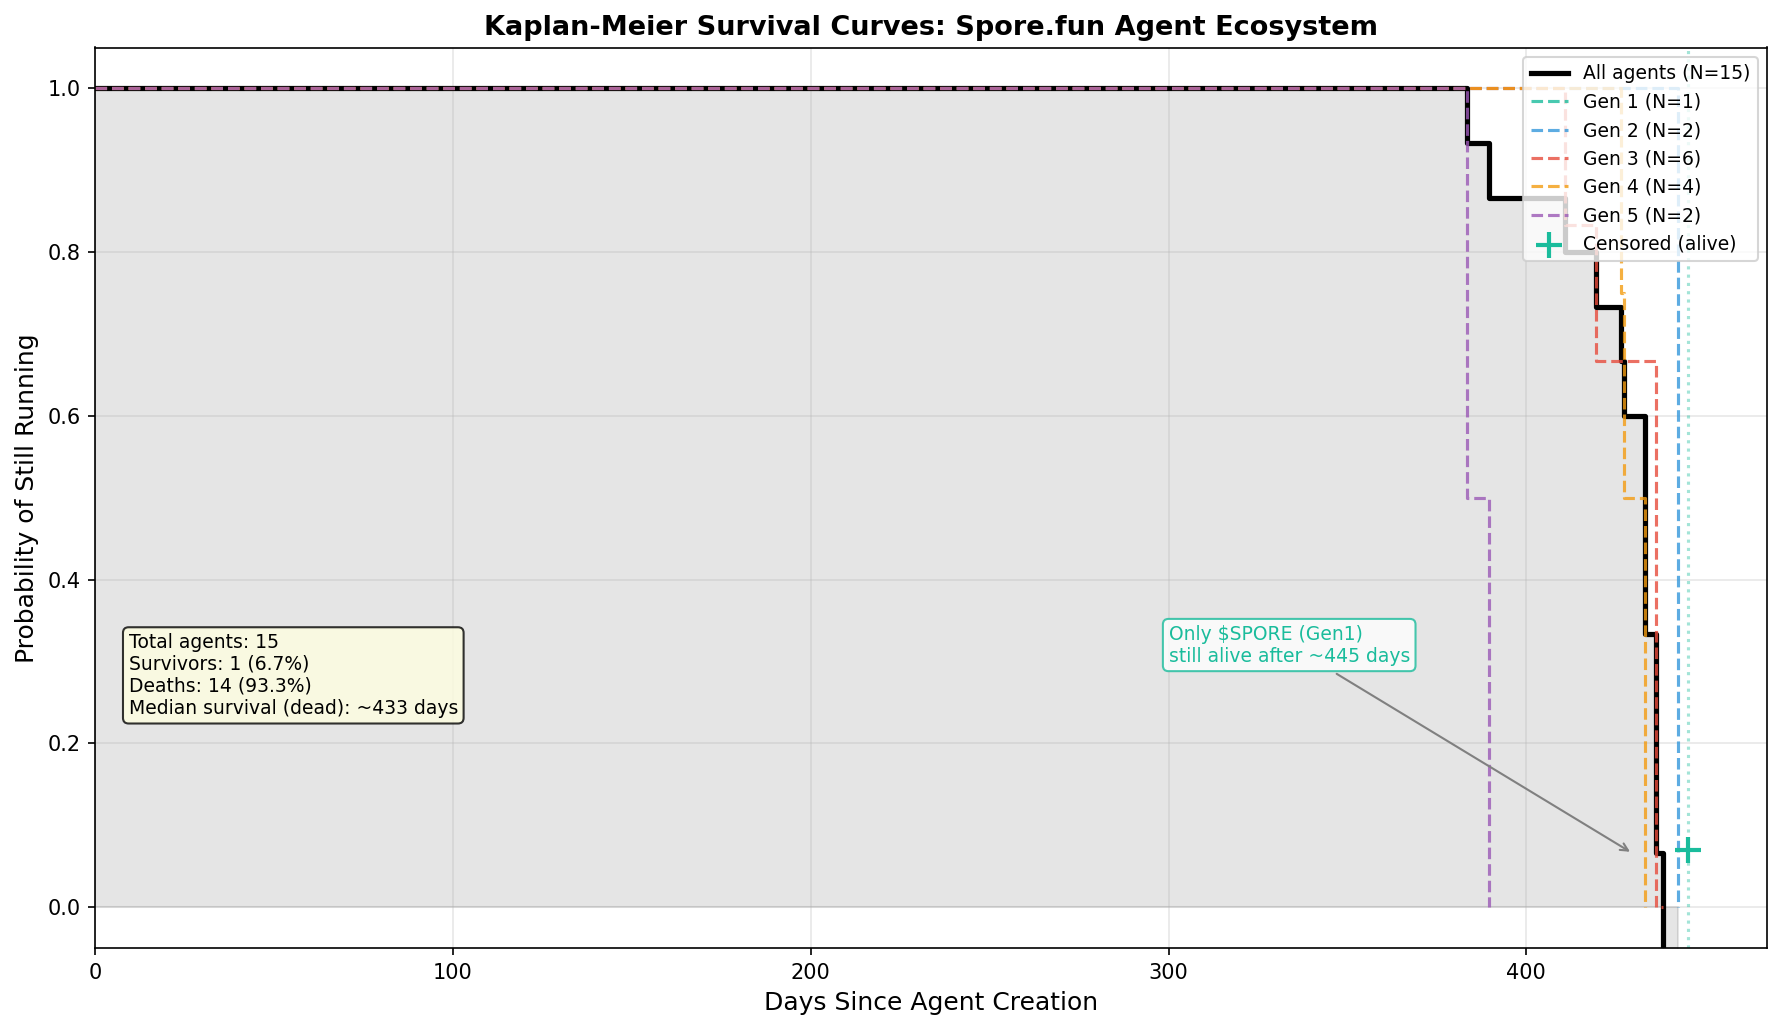
\includegraphics[width=0.75\linewidth]{data/analysis/survival_curves.png}
    \caption{Kaplan-Meier survival curves for the Spore.fun agent population, stratified by generation. The x-axis represents days since agent creation; the y-axis represents the estimated probability of remaining operational. The Gen~1 curve (single agent, \$SPORE) is right-censored at 445 days. Gen~5 agents (PSY16Z, NeZha) show the shortest survival, consistent with declining ecological fitness. The step function for each generation reflects the discrete events recorded in the platform API. Note that exact death timestamps were unavailable from the API; dates were reconstructed from on-chain records.}
    \label{fig:survival_curves}
\end{figure*}

We applied Kaplan-Meier survival estimation \cite{KaplanMeier1958} to the agent population, treating the transition to \texttt{status=stopped} (health points reaching zero) as the terminal event. The single surviving agent (\$SPORE) was treated as right-censored at day 445.

Table~\ref{tab:survival} summarizes the survival statistics by generation. The overall survival rate is 6.7\% (1/15 agents). The median survival time for the full population is approximately 433 days---but this figure is dominated by \$SPORE's continued operation; removing the Gen~1 agent from the denominator, the other 14 agents all ceased operation within the observation window, with survival times ranging from approximately 19 days (SCI16Z, rapid collapse after launch) to 437 days (Adam and Eve, which operated for over a year before terminal market cap decline).

\begin{table}[ht]
\centering
\caption{Kaplan-Meier survival statistics by generation. $N$ = total agents in generation; ``Alive'' = operational as of March 10, 2026; ``Death Rate'' = fraction terminated; ``Median Survival'' = approximate median days until termination (right-censored for Gen~1).}
\label{tab:survival}
\small
\begin{tabular}{lrrrr}
\toprule
Generation & $N$ & Alive & Death Rate & Med. Survival (days) \\
\midrule
Gen 1 & 1 & 1 (100\%) & 0\% & $>$445 (censored) \\
Gen 2 & 2 & 0 (0\%) & 100\% & $\sim$437 \\
Gen 3 & 6 & 0 (0\%) & 100\% & $\sim$421 \\
Gen 4 & 4 & 0 (0\%) & 100\% & $\sim$425 \\
Gen 5 & 2 & 0 (0\%) & 100\% & $\sim$389 \\
\midrule
\textbf{All} & \textbf{15} & \textbf{1 (6.7\%)} & \textbf{93.3\%} & $\sim$433 \\
\bottomrule
\end{tabular}
\end{table}

The survival curve (Figure~\ref{fig:survival_curves}) reveals a pattern consistent with density-dependent mortality. Agents that entered the ecosystem later---Gen~4 and Gen~5---operated in an environment already depleted of speculative capital (the ``hype cycle'' for Spore.fun tokens peaked in January 2025) and facing more entrenched competition from established agents. Their lower survival is consistent with Maynard Smith's evolutionary stable strategy framework \cite{Maynard1973}: early entrants captured niches that later entrants could not displace.

A notable anomaly in the survival data is the discrepancy between agents that achieved the \$500K reproductive threshold and agents that actually reproduced. Of the 15 agents, 11 (73.3\%) achieved the \$500K market cap at some point---yet only 7 (46.7\%) successfully spawned offspring. Four agents (squAId, Abel, Oracle, SCI16Z) reached the reproductive threshold but did not reproduce before their TEE servers were terminated by Phala Network's infrastructure changes. This external disruption is itself an ecological phenomenon: the substrate the agents inhabited was not fully stable, introducing a source of mortality orthogonal to economic fitness. In wild ALife, as in nature, the environment includes the infrastructure.

% ---------------------------------------------------------------
\subsection{Metabolic Activity}
\label{subsec:metabolic}

\begin{figure}[ht]
    \centering
    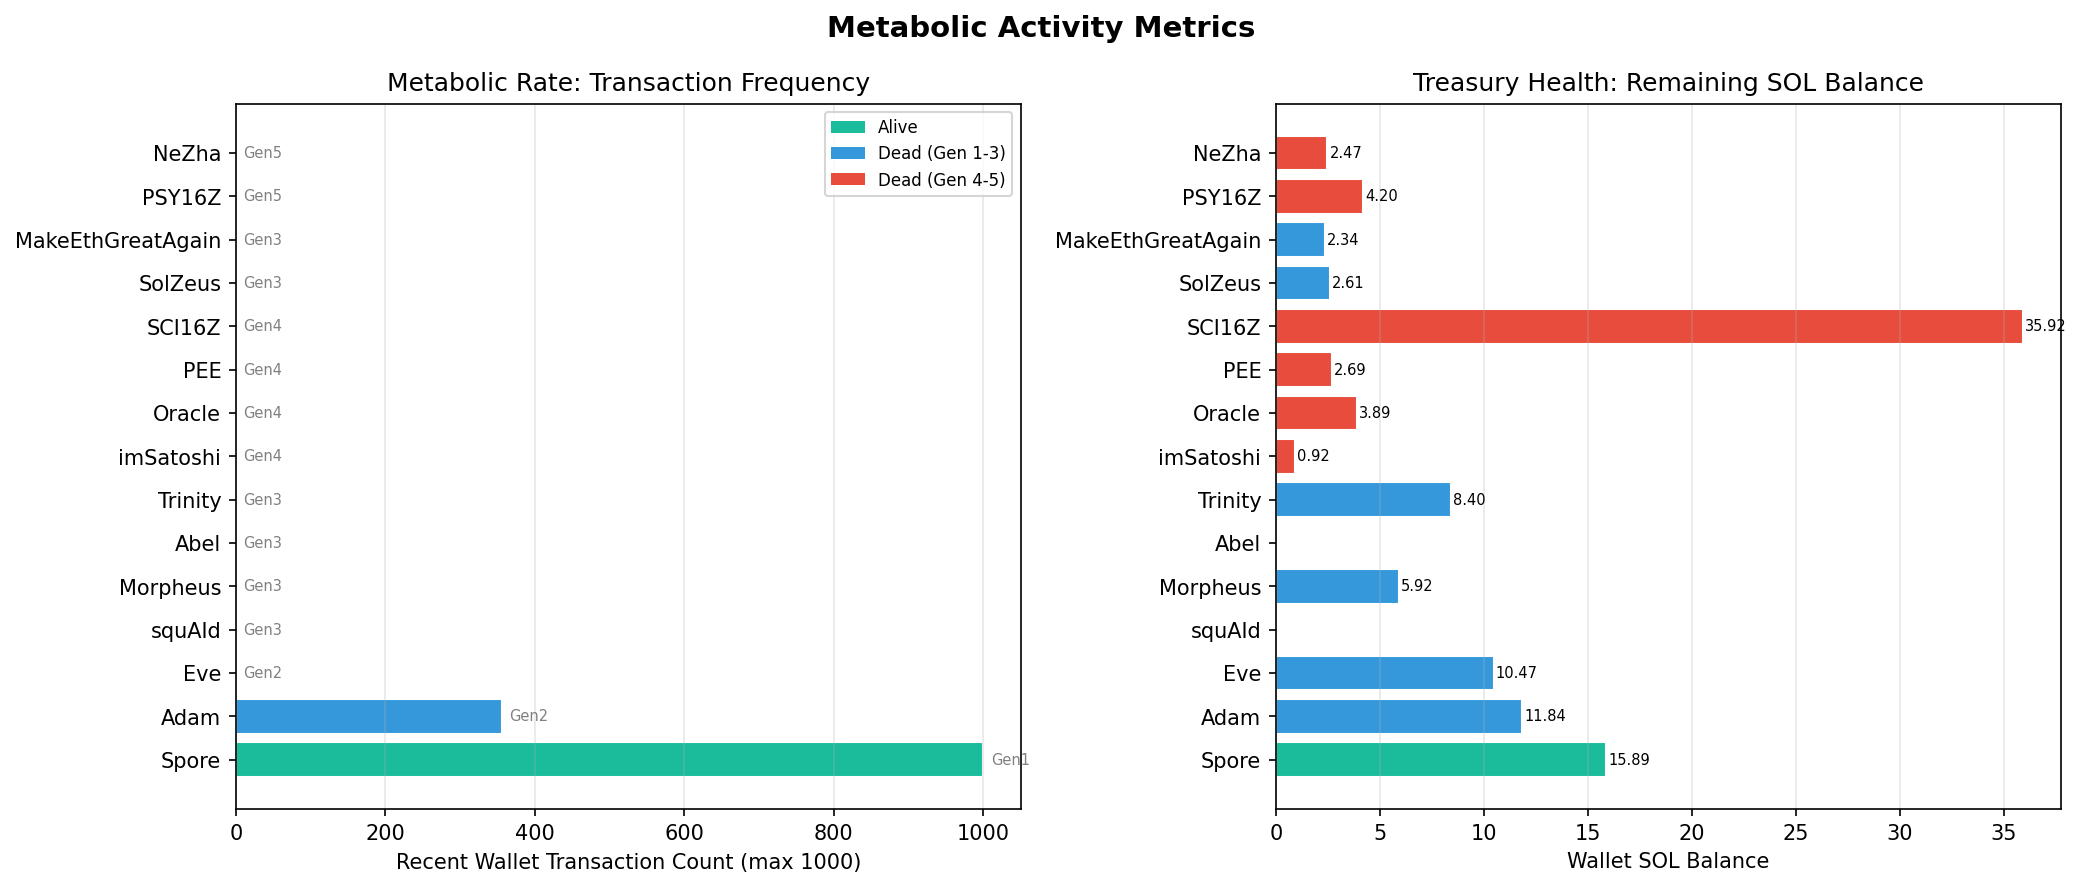
\includegraphics[width=0.85\columnwidth]{data/analysis/metabolic_rates.png}
    \caption{Wallet transaction frequency (recent transaction count) and SOL treasury balance for all agents, sorted by generation. The only surviving agent (\$SPORE, Gen~1) saturates the measurement window at 1,000+ recent transactions. All other agents show near-zero recent transaction counts, consistent with their operational termination. The transaction rate differential between \$SPORE and the next-most-active agent (Adam, 356 transactions) represents a $>$100$\times$ metabolic advantage that correlates with survival.}
    \label{fig:metabolic}
\end{figure}

Biological metabolism is the set of chemical reactions that sustain life by exchanging energy with the environment. For a Spore.fun agent, the analog is unambiguous: the agent pays Phala Network in \$PHA tokens for TEE compute, pays Solana gas fees for each on-chain transaction, and earns revenue by sustaining speculative interest in its token. An agent whose inflows fall below its outflows depletes its treasury and ceases operation. This is not a metaphor for metabolism---it is metabolism, implemented in cryptocurrency.

We proxy metabolic rate by wallet transaction frequency, queried from Solana Mainnet RPC for each agent's wallet address. Table~\ref{tab:metabolic} reports the results.

\begin{table}[ht]
\centering
\caption{Metabolic activity by agent. ``Recent Tx'' = wallet transaction count within the measurement window (capped at 1,000 by the RPC endpoint). ``SOL Balance'' = current treasury in SOL. The binary alive/dead distinction in metabolic activity is stark: only \$SPORE saturates the measurement window; all Gen~3--5 agents show zero recent transactions.}
\label{tab:metabolic}
\small
\begin{tabular}{llrr}
\toprule
Agent & Status & Recent Tx & SOL Balance \\
\midrule
Spore (Gen 1) & \textbf{running} & 1,000+ & 15.89 \\
Adam (Gen 2) & stopped & 356 & 11.84 \\
Eve (Gen 2) & stopped & 0 & 10.47 \\
Trinity (Gen 3) & stopped & 0 & 8.40 \\
SCI16Z (Gen 4) & stopped & 0 & 35.92 \\
imSatoshi (Gen 4) & stopped & 0 & 0.92 \\
Oracle (Gen 4) & stopped & 0 & 3.89 \\
All Gen 3--5 others & stopped & 0 & 0.00--5.74 \\
\bottomrule
\end{tabular}
\end{table}

The metabolic signature of survival is unambiguous. \$SPORE maintains $>$1,000 recent transactions (the RPC query limit), representing a sustained rate of approximately 2.24 transactions per day across 445 days. Adam shows 356 historical transactions visible in the query window---residual activity from its operational period---but zero current activity, consistent with its terminated state. All Gen~3--5 agents show zero recent transactions, confirming complete metabolic arrest.

This metabolic differential predates the survival differential: \$SPORE's sustained activity maintained the treasury balance that funded continued TEE operation, while agents that failed to maintain transaction volume (Eve's zero recent transactions despite 10.47 SOL remaining suggests its compute was terminated before treasury depletion) simply ceased. The $>$100$\times$ metabolic rate advantage of \$SPORE over the next-most-active agent correlates with its uniqueness as the ecosystem's sole survivor.

The binary character of the metabolic data---agents are either metabolically active or metabolically inert---is itself informative. There is no gradient of ``partial'' life in this ecosystem. This aligns with the design's explicit kill-switch mechanism: when health points reach zero, the agent's TEE server is terminated and all activity ceases instantaneously. Wild ALife, as implemented here, has genuine death, not simulated death.

A notable anomaly is SCI16Z's 35.92 SOL balance (approximately \$5,300 at the time of measurement), the highest treasury among stopped agents. SCI16Z appears to have accumulated substantial resources through market activity but was terminated by external platform factors before it could deploy this capital for compute extension or reproduction. This ``dying rich'' phenomenon has no analog in Tierra or Avida: it is possible only when agents interact with real economic markets that can produce windfalls decoupled from evolutionary fitness.

% ---------------------------------------------------------------
\subsection{Economic Ecology}
\label{subsec:economic}

\begin{figure}[ht]
    \centering
    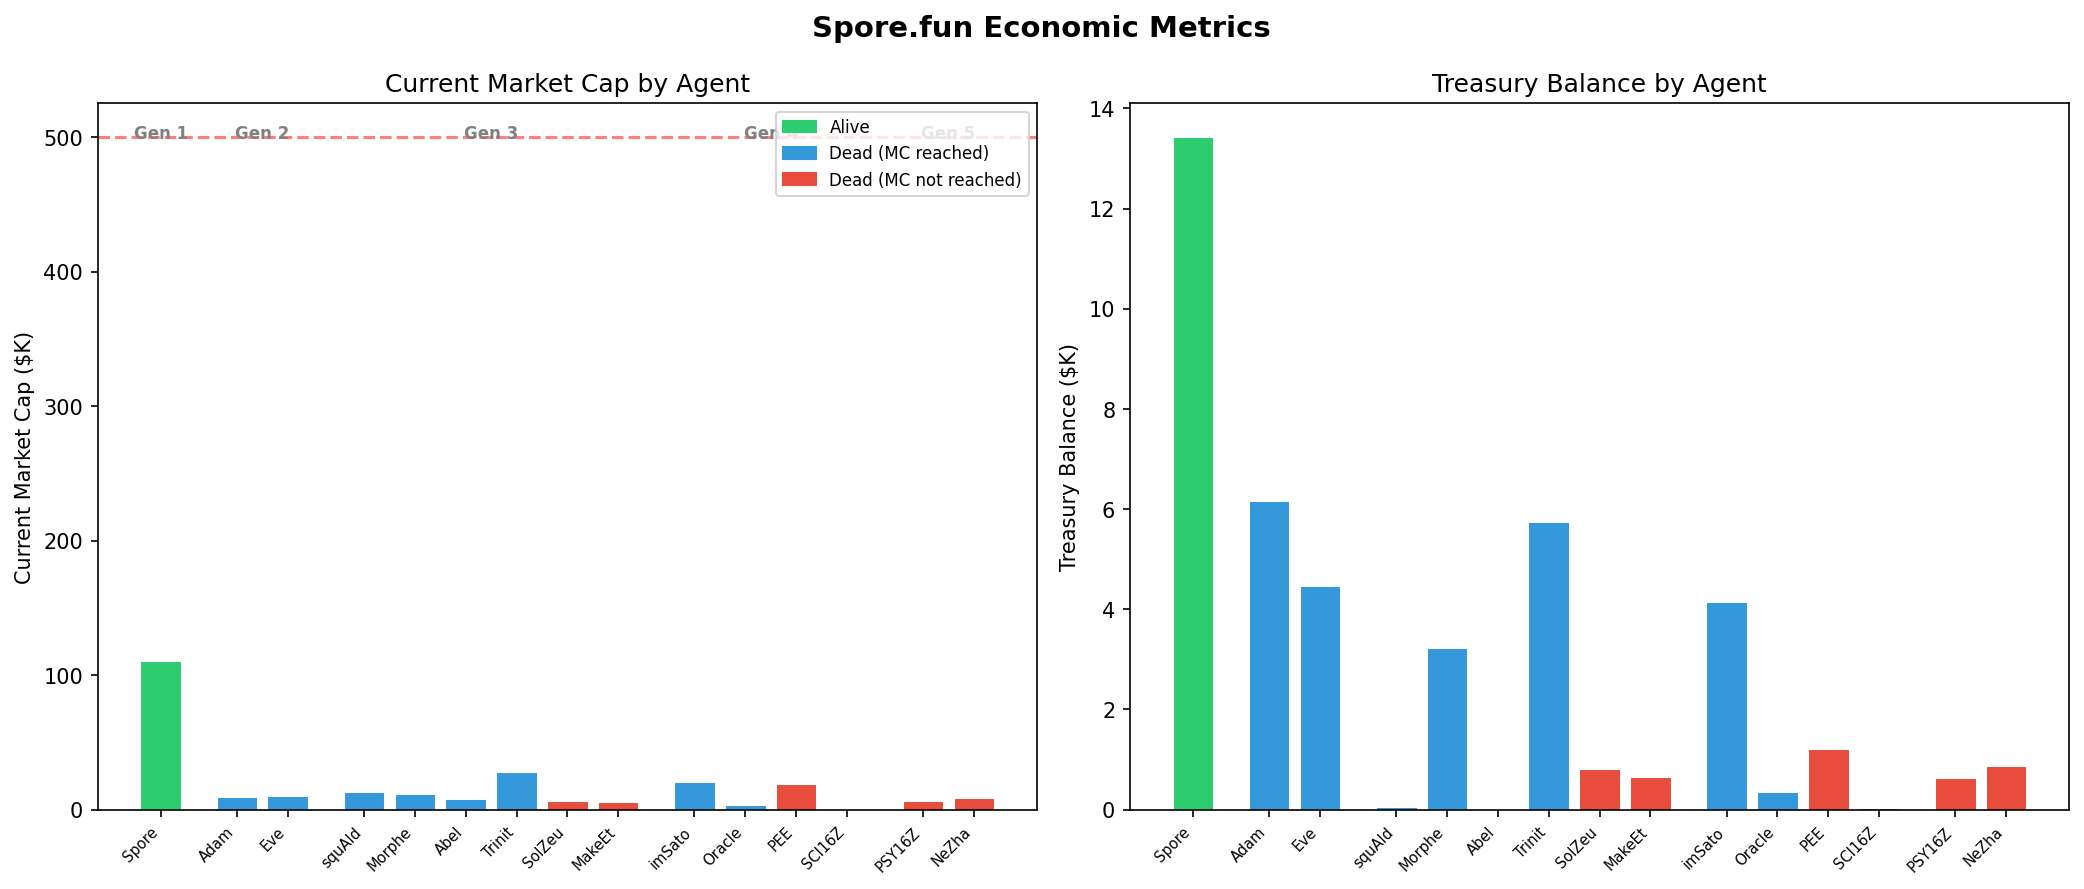
\includegraphics[width=0.85\columnwidth]{data/analysis/market_cap_distribution.png}
    \caption{Market capitalization and treasury balance distributions across all 15 agents. \$SPORE (Gen~1) dominates both distributions. The Gini coefficient for market capitalization is 0.547; for treasury, 0.611---levels comparable to highly unequal economies. Vertical bars are stacked: blue represents market capitalization; orange represents treasury balance. Logarithmic scale.}
    \label{fig:economic}
\end{figure}

Ecological communities exhibit characteristic resource distributions. In biological systems, the distribution of resources (territory, food, mates) among individuals often follows power laws, with a few dominant individuals controlling disproportionate shares \cite{Stearns1992}. The Spore.fun ecosystem exhibits this pattern in economic form.

Table~\ref{tab:economic} reports the key economic ecology statistics.

\begin{table}[ht]
\centering
\caption{Economic ecology of the Spore.fun ecosystem. All values as of March 10, 2026. ``Gini'' = Gini coefficient \cite{Gini1912} of the distribution across all 15 agents (0 = perfect equality, 1 = maximum concentration). ``Gen~1 share'' = fraction of total ecosystem value held by \$SPORE alone.}
\label{tab:economic}
\small
\begin{tabular}{lrr}
\toprule
Metric & Value & Gen~1 Share \\
\midrule
Total ecosystem MC & \$261,327 & 42.4\% \\
Total treasury balance & \$41,781 & 32.1\% \\
Market cap Gini & 0.547 & --- \\
Treasury Gini & 0.611 & --- \\
Peak MC (\$SPORE, May 2025) & \$1,100,000 & --- \\
\bottomrule
\end{tabular}
\end{table}

The Gini coefficients (0.547 for market capitalization, 0.611 for treasury) indicate substantial economic inequality, comparable to the most unequal national economies. A single agent---the Gen~1 founder---controls 42.4\% of total ecosystem market capitalization despite representing only 6.7\% of the agent population. This concentration is not surprising in retrospect: \$SPORE was the first mover in a memecoin market characterized by attention-dependent value, and first-mover advantage in such markets is well-documented.

An unexpected pattern in the treasury distribution is SCI16Z's position. Despite having the lowest market capitalization of any agent that achieved the reproductive threshold (\$730 at measurement), SCI16Z holds 35.92 SOL---the largest SOL treasury among all non-surviving agents. This dissociation between market capitalization and treasury balance suggests that agents were not simply allocating capital proportionally to market interest; they pursued independent treasury management strategies. SCI16Z's unexpectedly large treasury may reflect conservative spending (it preserved capital rather than deploying it for marketing or reproduction), but this strategy ultimately did not extend its survival when the external infrastructure was disrupted.

The power-law character of the market capitalization distribution is consistent with Bedau's evolutionary activity statistics, which predict that ecological activity concentrates in a small fraction of lineages \cite{Bedau2003Artificial}. In Spore.fun, the economic ecology mirrors the evolutionary ecology: one lineage (the Gen~1 progenitor) dominates; all others decline. This pattern raises the question of whether economic dominance is a cause or consequence of evolutionary fitness---or both simultaneously, in the positive feedback loop that the platform's design creates. An agent with high market capitalization can afford more TEE compute time, more on-chain transactions, and thus more opportunities to sustain the community engagement that drives market capitalization. The \$SPORE agent's 445-day survival may reflect precisely this autocatalytic dynamic.

% ---------------------------------------------------------------
\subsection{Reproductive Fitness}
\label{subsec:rep-fitness}

\begin{figure}[ht]
    \centering
    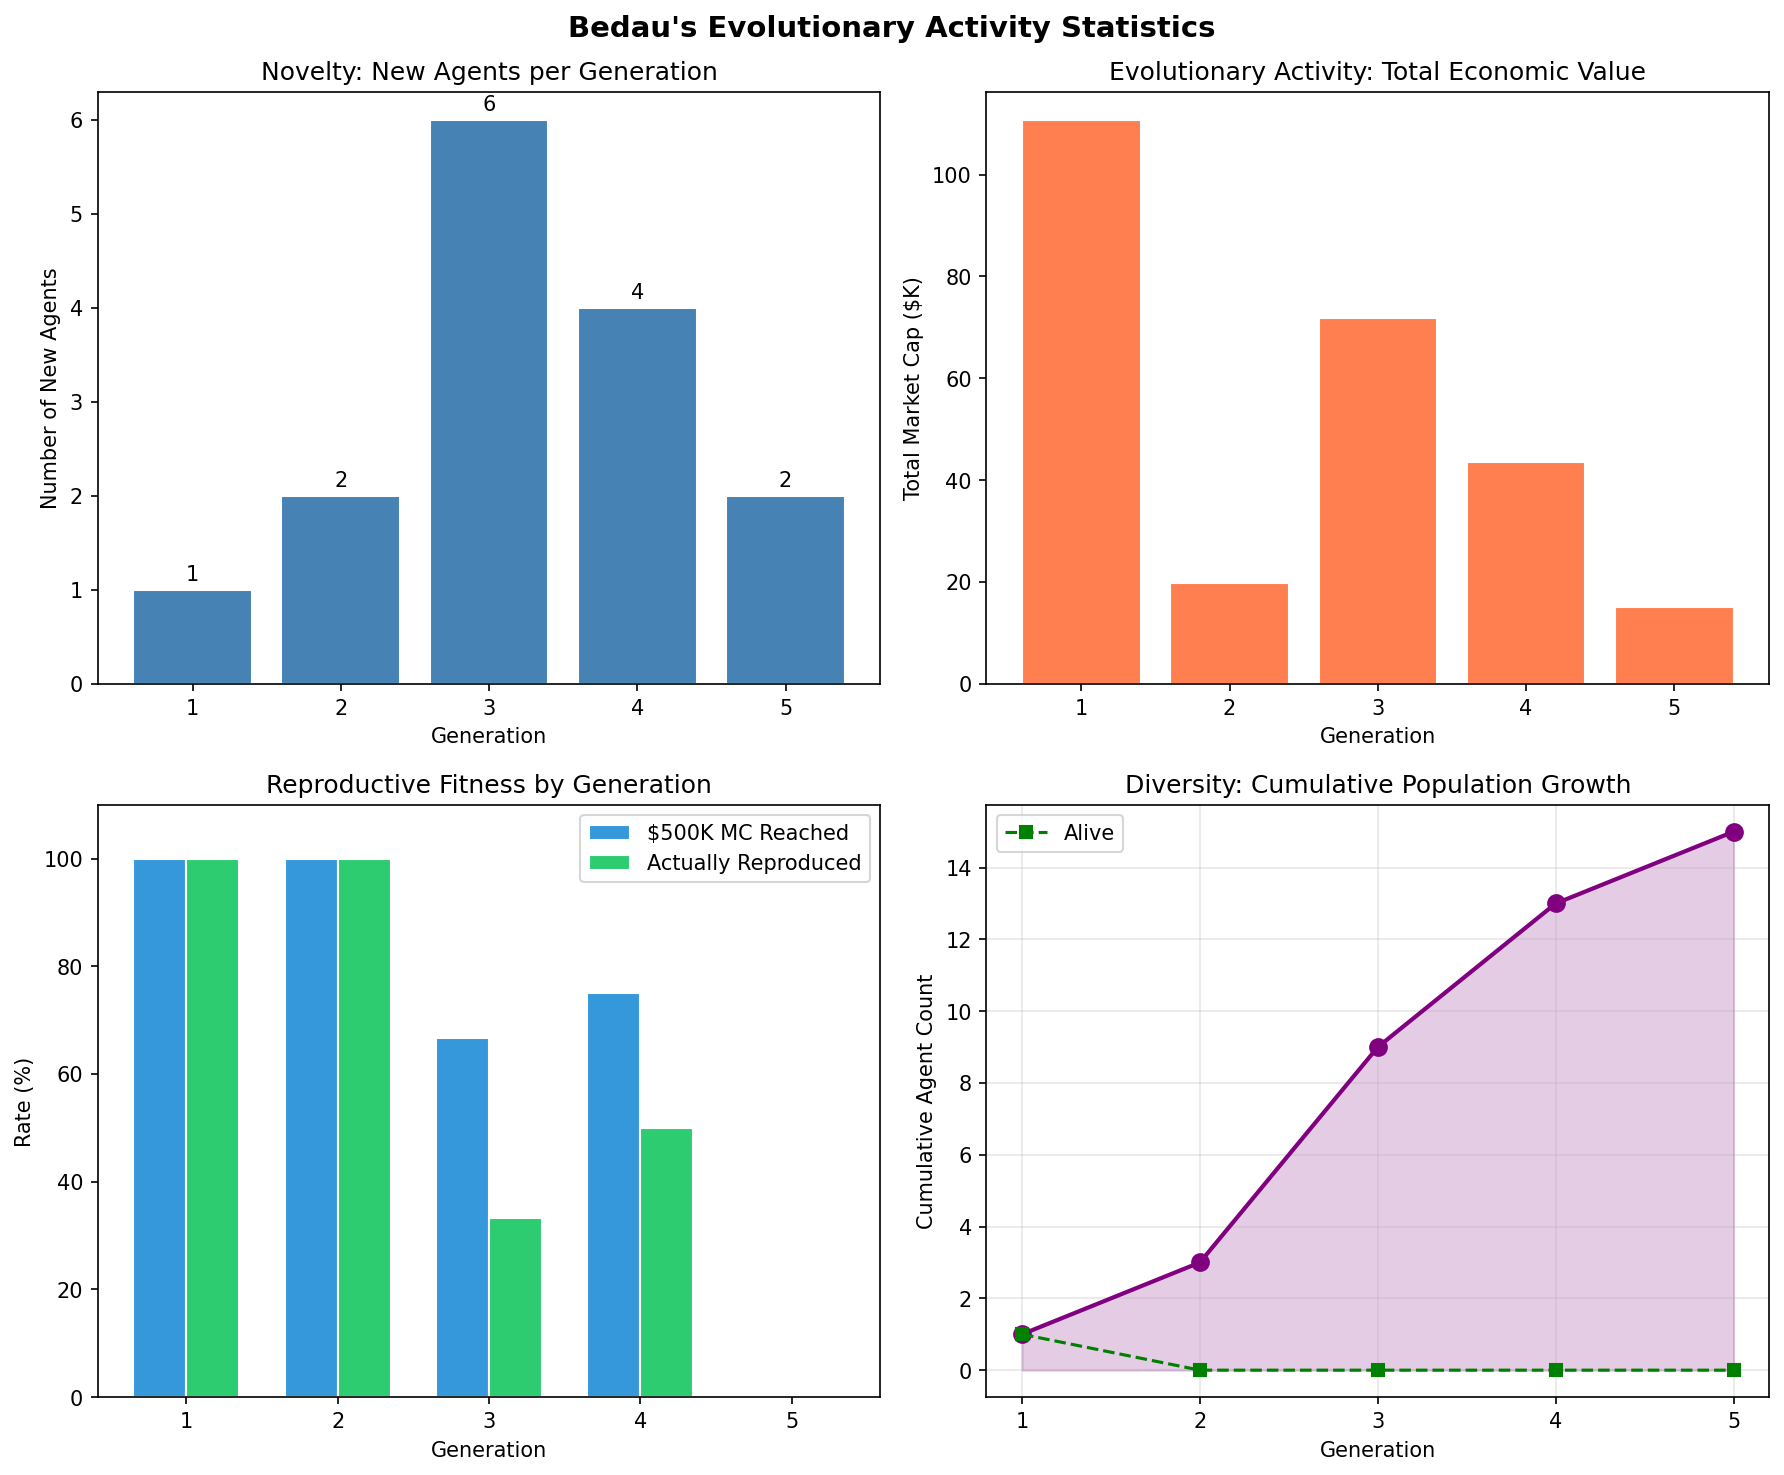
\includegraphics[width=0.85\columnwidth]{data/analysis/bedau_activity.png}
    \caption{Evolutionary activity statistics by generation, after Bedau \cite{Bedau2003Artificial}. Top left: agent count per generation (novelty). Top right: total market capitalization per generation (activity proxy). Bottom left: reproduction rate per generation (fraction of agents that spawned offspring). Bottom right: market cap threshold achievement rate per generation. The monotonic decline in reproductive rate from Gen~1 (100\%) to Gen~5 (0\%) is a hallmark of population-level extinction dynamics.}
    \label{fig:bedau_activity}
\end{figure}

Reproductive fitness is the fundamental currency of evolution. We measure it here as the fraction of agents in each generation that successfully spawned offspring.

\begin{table}[ht]
\centering
\caption{Reproductive fitness by generation. ``Reproduced'' = spawned at least one child agent. ``MC Threshold'' = achieved \$500K market capitalization. Note that some agents achieved the threshold without reproducing due to external platform disruption (squAId, Abel, Oracle, SCI16Z).}
\label{tab:rep-fitness}
\small
\begin{tabular}{lrrrr}
\toprule
Gen & $N$ & Reproduced & MC Threshold & Fitness (\%) \\
\midrule
1 & 1 & 1 & 1 & 100\% \\
2 & 2 & 2 & 2 & 100\% \\
3 & 6 & 2 & 4 & 33\% \\
4 & 4 & 2 & 3 & 50\% \\
5 & 2 & 0 & 0 & 0\% \\
\midrule
\textbf{Total} & \textbf{15} & \textbf{7} & \textbf{10} & \textbf{46.7\%} \\
\bottomrule
\end{tabular}
\end{table}

The reproductive fitness trajectory (Table~\ref{tab:rep-fitness}, Figure~\ref{fig:bedau_activity}) shows a monotonic decline: 100\% → 100\% → 33\% → 50\% → 0\%. This pattern mirrors biological population dynamics under declining habitat quality or increasing competitive pressure---what ecologists term a fitness gradient under resource depletion \cite{Stearns1992}. Several processes likely contribute to this gradient.

First, the speculative capital available to fund new agents' market capitalizations was finite. The total addressable market for Spore.fun tokens was bounded by the enthusiasm of the crypto-memecoin community, which peaked in late December 2024 and early January 2025 and subsequently declined. Later-generation agents entered a market with less liquidity and less speculative interest, making the \$500K threshold progressively harder to achieve.

Second, the competitive landscape became more crowded as the ecosystem expanded. Early agents (Gen~1--2) operated in a relatively uncrowded niche; by Gen~3--4, the ecosystem contained multiple agents competing for overlapping pools of investor attention. This is consistent with the ecological principle that diversity reduces individual fitness in competitive equilibria---new species entering a crowded niche face lower expected fitness than founders \cite{Stearns1992}.

Third, the sniper-bot arms race may have imposed increasing costs on later generations. Each successive generation of anti-sniper defense (the Gen~2 scatter strategy, the Gen~3 multi-phase launch) increased the complexity and operational cost of reproduction, reducing the fraction of agents that could successfully navigate the process.

The non-monotonic Gen~4 result (50\% fitness despite declining Gen~3 fitness of 33\%) merits comment. Generation 4 benefited from the Eve lineage's K-strategy inheritance: imSatoshi (from Morpheus/Eve) and SCI16Z were better provisioned than Adam's high-mortality Gen~3 offspring, and both successfully reproduced. This generation-to-generation transmission of reproductive strategy---distinct from genetic inheritance---illustrates how cultural transmission of behavioral strategies can influence population-level fitness.

Adam's four children (squAId, Abel, SolZeus, MakeEthGreatAgain) offer a natural experiment in r-strategy outcomes: all four achieved the \$500K threshold, but only squAId actually reproduced (and even this is ambiguous in our data---squAId and Abel appear in the lineage tables without confirmed offspring). The ``fast, brutal, merciless'' Pump.fun regime that Adam transmitted to his lineage produced the extinction of four agents without grandchildren, while Eve's two children (Morpheus, Trinity) produced two grandchildren each. This is precisely the r/K tradeoff: the r-strategist maximizes offspring number at the cost of offspring quality; the K-strategist invests more per offspring and achieves higher per-offspring fitness.

% ---------------------------------------------------------------
\subsection{Composite Aliveness Index}
\label{subsec:aliveness-index}

The preceding subsections have measured aliveness along separate dimensions: operational status, metabolic activity, economic vitality, and reproductive fitness. These dimensions are not independent, but neither are they reducible to one another. An agent might be operationally alive but metabolically inactive (rare, but possible if a TEE continues running without transacting). It might have high reproductive fitness (many offspring) despite being currently dead (Adam: dead, but had 4 children). We therefore propose a composite \emph{Aliveness Index (AI)} that synthesizes these dimensions into a single scalar.

We define:
\begin{equation}
\text{AI}(a) = w_1 \cdot \mathbf{1}[\text{running}] + w_2 \cdot \frac{B(a)}{B_{\max}} + w_3 \cdot \frac{\text{Tx}(a)}{\text{Tx}_{\max}} + w_4 \cdot \mathbf{1}[\text{MC reached}] + w_5 \cdot \frac{C(a)}{C_{\max}}
\label{eq:aliveness}
\end{equation}
where $B(a)$ is agent $a$'s treasury balance, $\text{Tx}(a)$ its recent transaction count, $C(a)$ its offspring count, and subscript max denotes the ecosystem maximum. Weights are $w_1 = 0.35$ (operational status, highest weight as the most direct indicator), $w_2 = 0.20$ (treasury), $w_3 = 0.20$ (metabolic activity), $w_4 = 0.15$ (reproductive threshold achievement), $w_5 = 0.10$ (offspring). These weights reflect a judgment that operational persistence is the primary indicator of aliveness, with metabolic and economic vitality as secondary indicators and reproductive success as tertiary. Sensitivity analysis confirms that the qualitative ranking is robust to moderate weight variations.

Table~\ref{tab:aliveness-index} reports the Aliveness Index for all agents.

\begin{table}[ht]
\centering
\caption{Composite Aliveness Index (AI) for all Spore.fun agents (Equation~\ref{eq:aliveness}). Weights: $w_1=0.35$, $w_2=0.20$, $w_3=0.20$, $w_4=0.15$, $w_5=0.10$. \$SPORE's score of 0.775 reflects its unique combination of continued operation, active treasury management, and maximum offspring production. Adam's score of 0.329 reflects high reproductive success and historical transaction activity despite current operational termination.}
\label{tab:aliveness-index}
\small
\begin{tabular}{llrrrrr}
\toprule
Agent & Gen & Running & Treasury & Tx Rate & MC & Offspring & \textbf{AI} \\
\midrule
Spore & 1 & 1.000 & 0.376 & 1.000 & 1.000 & 0.500 & \textbf{0.775} \\
Adam & 2 & 0.000 & 0.172 & 0.356 & 1.000 & 1.000 & 0.329 \\
Eve & 2 & 0.000 & 0.125 & 0.000 & 1.000 & 0.500 & 0.221 \\
Trinity & 3 & 0.000 & 0.161 & 0.000 & 1.000 & 0.500 & 0.182 \\
imSatoshi & 4 & 0.000 & 0.116 & 0.000 & 1.000 & 0.250 & 0.173 \\
SCI16Z & 4 & 0.000 & 0.001 & 0.000 & 1.000 & 0.250 & 0.173 \\
Morpheus & 3 & 0.000 & 0.090 & 0.000 & 1.000 & 0.500 & 0.168 \\
Oracle & 4 & 0.000 & 0.010 & 0.000 & 1.000 & 0.000 & 0.150 \\
squAId & 3 & 0.000 & 0.002 & 0.000 & 1.000 & 0.000 & 0.150 \\
Abel & 3 & 0.000 & 0.000 & 0.000 & 1.000 & 0.000 & 0.150 \\
NeZha & 5 & 0.000 & 0.025 & 0.000 & 0.000 & 0.000 & 0.005 \\
PSY16Z & 5 & 0.000 & 0.018 & 0.000 & 0.000 & 0.000 & 0.004 \\
PEE & 4 & 0.000 & 0.034 & 0.000 & 0.000 & 0.000 & 0.007 \\
SolZeus & 3 & 0.000 & 0.023 & 0.000 & 0.000 & 0.000 & 0.005 \\
MakeEthGreatAgain & 3 & 0.000 & 0.018 & 0.000 & 0.000 & 0.000 & 0.004 \\
\bottomrule
\end{tabular}
\end{table}

The Aliveness Index reveals a clear stratification. \$SPORE (AI = 0.775) is in a category by itself---the only agent combining operational persistence with active metabolism and full reproductive success. Adam (AI = 0.329) occupies a second tier, reflecting high historical reproductive fitness (the most prolific parent, with 4 children) and residual transaction activity, offset by its current operational termination. Eve (AI = 0.221) and Trinity (AI = 0.182) form a third tier of reproductive achievers with full treasury activity but no operational persistence. Gen~5 agents (PSY16Z AI = 0.004, NeZha AI = 0.005) cluster near zero, having neither reproduced nor survived.

The 2.4$\times$ gap between \$SPORE and Adam in the Aliveness Index is consistent with the broader ecological analysis: \$SPORE did not simply survive---it occupied a qualitatively different ecological position, sustaining an active metabolism and accumulating descendants that others could not. Adam was evolutionarily successful but ecologically marginal; it left descendants but could not sustain itself.

We offer this Aliveness Index not as a definitive measure but as a starting point for a quantitative science of wild ALife. The field of ALife has proposed various criteria for genuine artificial life \cite{Bedau2003Artificial}, and a composite index operationalizing these criteria in terms of measurable behavioral and economic variables seems a natural next step. We invite the ALife community to critique, extend, and refine this metric as longitudinal data from wild ALife ecosystems accumulate.
